\chapter{Návrh řešení} % TODO lepe promyslet jak se ujmout teto casti
\label{Koncept reseni}
%popis jednotlivych bloku realizace, s odkazem na blokove schema z Kapitoly 3
Návrh řešení musí brát ohled na primární požadavky, které zařízení musí splňovat, aby byla zajištěna základní funkčnost zařízení. Prvním primárním požadavkem, je zajištění základní funkčnosti detektoru Timepix 2, tyto požadavky byly popsány v části \ref{Technicka specifikace}. Dalším požadavkem na navrhované vyčítací rozhraní je jeho celková miniaturizace, tento požadavek stanovuje zadní diplomové práce.
\par Podrobnější rozbor celkového řešení této práce, je dále v části \ref{realizace}, kde bude popsán výběr konkrétních součástek a návrh zapojení rozhraní, respektující primární požadavky uvedené v této části textu \ref{Koncept reseni}.

\section{Koncept řešení}
Navržený koncept vyčítacího rozhraní je zobrazen pomocí schematického nákresu na obrázku \ref{fig:navrh_reseni}. Koncept rozhraní se skládá ze dvou desek plošných spojů (PCB). 
\par První deskou plošných spojů je deska s označením \textit{základní deska} \ref{fig:navrh_reseni}. Na této desce je implementováno většina funkcionalit potřebných pro komunikaci s detektorem Timepix 2. Dále je zde implementována USB komunikace, která slouží pro komunikaci s u  uživatelským rozhraní přes USB.
\par Druhou deskou plošných spojů je deska s názvem \textit{chipboard} \ref{fig:navrh_reseni}. Na této desce se nachází samotný detektor Timepix 2. Dále je zde implementován vysokonapěťový zdroj (HV), měření vysokého napětí a měření teploty.

Toto rozložení bylo navrhnutu s ohledem na požadavky miniaturizace celého zařízení, a také s ohledem na variabilitu zařízení. Variabilitu ve smyslu možnosti připojit k jedné základní desce různé chipboardové desky, tento koncept lze také najít například v zařízení popsaném v části \ref{Katherine}. Dále byl koncept navrhnut s ohledem na možnost vyčítací rozhraní připojit k uživatelskému rozhraní, konkrétně k osobnímu počítači.  

\begin{figure}[h!]
	\centering
	\captionsetup{justification=centering}
	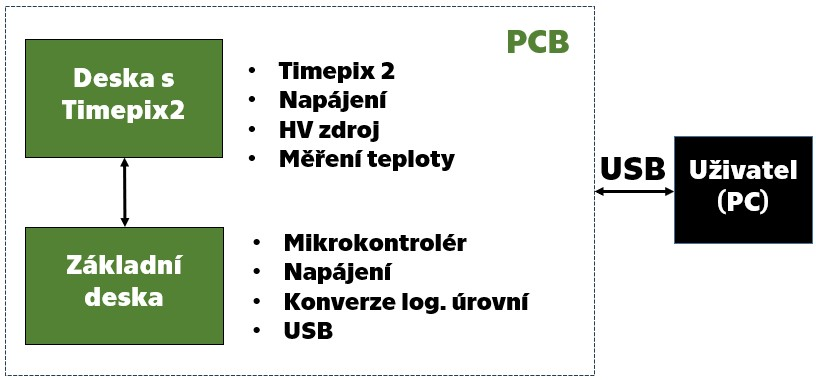
\includegraphics[scale=0.80]{navrh_reseni.jpg}
	\caption{Koncept řešení vyčítacího rozhraní pro detektor Timepix 2} 
	\label{fig:navrh_reseni}
\end{figure}

\subsection{Komunikace s Timepix 2}
Pro komunikaci s Timepix 2 je možné využít sériové, nebo paralelní rozhraní. jak již bylo zmíněno v části \ref{Komunikacni rozhrani}. Pro tuto práci uvažujme využití pouze sériové komunikace. Využití sériového rozhraní pro komunikaci s Timepix 2, umožní použít mikrokontrolér. Maximální vyčítací rychlost z detektoru Timepix 2 je 100 Mbits/s. S ohledem na tuto maximální rychlost vyčítaní dat z Timepix 2 musí být vybrán vhodný mikrokontrolér pro obsluhu komunikace, nejen s Timepix 2 detektorem. 

\subsection{Uživatelské rozhraní}
Uživatelské rozhraní pro tuto práci bylo zvoleno rozhraní USB s konektorem typu C. Použit byl standart USB 2.0 High Speed. Tento standart umožňuje komunikovat maximální rychlostí až 480 Mbit/s. S respektem na maximální rychlost vyčítání dat z detektoru Timepix 2, která je 100 Mbits/s, je tato rychlost dostačující. 

\subsection{Napájení}
Pro napájení detektoru Timepix 2 jsou dle \ref{tab:tpx2_napajeni} zapotřebí tři napájecí napětí. Napájecí zdroje musí být vhodné pro maximální odběr detektoru Timepix 2. Celková spotřeba samotného detektoru, by neměla být dle \ref{Timepix2} vyšší než něž 900 mW. 
\par Dalším potřebným napájením potřebným pro navržený koncept je napájení mikrokontroléru. Toto napájení je závislé na konkrétním typu mikrokontroléru. Detailnější informace o výběru mikrokontroléru a jeho potřebných napájecích úrovní budou v části \ref{realizace}. 

\subsection{Mechanika}
Návrh rozhraní je rozložen do dvou desek plošných spojů spojenými konektorem. Při návrhu mechanické části rozhraní musí být zajištěna mechanické odolnost vůči poškození, především nejcitlivější části \textit{wire bondů} \ref{fig:bga}. Dále musí být umožněno se připojit k rozhraní pomocí konektoru. V neposlední řadě musí být zajištěn odvod tepla ze součástek vyčítacího rozhraní, které mají největší výkon. Těmito objekty jsou především samotný detektor Timepix 2, mikrokontrolér a napájecí zdroje. 
